\tikzset{>=latex} % for LaTeX arrow head
\colorlet{Bcol}{violet!90}
\colorlet{BFcol}{red!60!black}
\colorlet{veccol}{green!45!black}
\colorlet{Icol}{blue!70!black}
\tikzstyle{BField}=[->,thick,Bcol]
\tikzstyle{current}=[->,Icol] %thick,
\tikzstyle{force}=[->,thick,BFcol]
\tikzstyle{vector}=[->,thick,veccol]
\tikzstyle{velocity}=[->,very thick,vcol]
\tikzstyle{charge+}=[very thin,draw=black,top color=red!50,bottom color=red!90!black,shading angle=20,circle,inner sep=0.5]
\tikzstyle{charge-}=[very thin,draw=black,top color=blue!50,bottom color=blue!80,shading angle=20,circle,inner sep=0.5]
\tikzstyle{metal}=[top color=black!15,bottom color=black!25,middle color=black!5,shading angle=10]
\tikzset{
  BFieldLine/.style={thick,Bcol,decoration={markings,mark=at position #1 with {\arrow{latex}}},
                                 postaction={decorate}},
  BFieldLine/.default=0.5,
  pics/Bin/.style={
    code={
      \def\R{0.12}
      \draw[pic actions,line width=0.6,#1] % ,thick
        (0,0) circle (\R) (-135:.75*\R) -- (45:.75*\R) (-45:.75*\R) -- (135:.75*\R);
  }},
  pics/Bout/.style={
    code={
      \def\R{0.12}
      \draw[pic actions,line width=0.6,#1,fill=white] (0,0) circle (\R);
      \fill[pic actions,#1] (0,0) circle (0.3*\R);
  }},
  pics/Bin/.default=Bcol,
  pics/Bout/.default=Bcol,
}

% CURRENT IN B FIELD


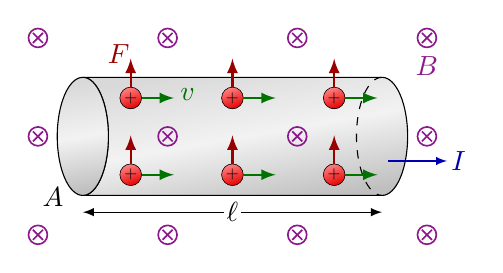
\begin{tikzpicture}
  \def\xmax{3.8}
  \def\ymax{1.25}
  \def\R{0.2}
  \def\Rx{0.26*\ymax}
  \def\Ry{0.6*\ymax}
  \def\L{\xmax}
  \def\NBy{3}
  \def\NBx{4}
  \coordinate (LT) at (0,\Ry);
  \coordinate (LB) at (0,-\Ry);
  \coordinate (RT) at (\L,\Ry);
  \coordinate (RB) at (\L,-\Ry);
  \coordinate (Q) at (0.15*\xmax,0.15*\ymax);
  \def\charge#1#2{
    \node[charge+,draw=black,circle,fill,inner sep=1,scale=0.6] (q) at (#1*\xmax,#2*\Ry) {$+$};
    \draw[vector] (q) --++ (0:0.55);
    \draw[force] (q) --++ (90:0.5);
  }
  
  % CURRENT
  \draw[metal]
    (LB) arc (-90:90:{\Rx} and {\Ry}) --
    (RT) arc (90:-90:{\Rx} and {\Ry}) -- cycle;
  \draw[metal] (0,0) ellipse ({\Rx} and {\Ry});
  \draw[dashed] (RT) arc (90:270:{\Rx} and {\Ry});
  %\draw[metal] (RT) arc (-90:90:{\Rx} and {\Ry});
  
  % CHARGE
  \charge{0.16}{0.65}
  \charge{0.50}{0.65}
  \charge{0.84}{0.65}
  \charge{0.16}{-.65}
  \charge{0.50}{-.65}
  \charge{0.84}{-.65}
  
  % B FIELD
  \foreach \i [evaluate={\y=(\i-\NBy/2-0.5)*2*\ymax/(\NBy-1);}] in {1,...,\NBy}{
    \foreach \j [evaluate={\x=-0.15*\xmax+(\j-1)*1.3*\xmax/(\NBx-1);}] in {1,...,\NBx}{
      \pic at (\x,\y) {Bin};
    }
  }
  \node[Bcol] at (1.15*\xmax,0.71*\ymax) {$\vb{B}$};
  \node at (-0.1*\xmax,-1.02*\Ry) {$A$};
  \node[BFcol] at (0.12*\xmax,1.4*\Ry) {$\vb{F}$};
  \node[veccol] at (0.35*\xmax,0.70*\Ry) {$\vb{v}$};
  \draw[<->] (LB)++(-90:0.17*\ymax) --++ (\L,0) node[midway,fill=white,inner sep=1] {$\ell$};
  \draw[current] (1.02*\xmax,-0.25*\ymax) --++ (0.6*\ymax,0) node[right=-2] {$I$};
  
\end{tikzpicture}
